\documentclass[12pt]{article}
\setlength\parindent{0pt}
\setlength\parskip{0.2cm}
\usepackage[margin=1in]{geometry}
\usepackage[utf8]{inputenc}
\usepackage{listings}
\usepackage{parcolumns}
\usepackage{appendix}
\usepackage{graphicx}
\lstset{
    numbers=left,
    breaklines=true,
    tabsize=2,
    basicstyle=\footnotesize\ttfamily,
    literate={\ \ }{{\ }}1
}

\begin{document}
\begin{titlepage}
    \begin{center}
    
        \vspace*{1cm}
    
        \textbf{Arm RSA Encryption}
    
        \vspace{2.0cm}
    
        \textbf{Zachary Dirk}
        
        \vfill
    
        Submission date: August 6th, 2019

        In affiliation with the UVic Department of Computer Science
    
        \vspace{0.8cm}
        
    \end{center}
\end{titlepage}

\tableofcontents

\clearpage

\section{Introduction}

RSA encryption is a common encryption algorithm in use today. The security of RSA is hinged upon the difficulty of factoring a product of two large prime numbers. A key component of the RSA algorithm is modular exponentiation, as the encryption itself is simply raising the message to the power of the public key mod M, while decryption is raising the ciphertext to the power of the private key mod M, where M is the previously mentioned product of primes. Trying to perform modular exponentiation in an embedded space can be difficult as the algorithm itself is quite expensive; the numbers can grow quite large. For this reason, care must be taken to optimize the RSA algorithm. An algorithm to accomplish this is montgomery modular multiplication (MMM). MMM is an algorithm for efficiently computing $X \cdot Y\ mod\ M$ and can be used in modular exponentiation by repeatedly using MMM with $X = Y$. In this report I will discuss my implementation of an efficient RSA encryption program in C, and what optimization techniques I used to try and make it even quicker. Lastly I will discuss my results and compare them to GCC's optimization results.

\section{Theoretical Background}

In this section I intentionally skip over the RSA key generation and focus exclusively on MMM as in my own implementation I made concessions to make that part simple. This allowed me to focus wholly on optimizing the MMM aspect of the algorithm.

If performed in the traditional sense, multiply then modulus, modular exponentiation is very slow as the numbers will grow incredibly large before they're reined in. MMM as presented in RSA \& Public Key Cryptography in FPGAs is a means to achieve a scalable and efficient implementation of RSA encryption \cite{RSA}. The big gain in the algorithm is converting the modulus operation into a series of additions, multiplications, and a right shift. Modulus itself is actually three operations: a subtraction, a multiplication, and a division, and the division is what makes it so expensive. By substituting the division with a right shift it's possible to save incredible amounts of resources. The algorithm presented in the paper is presented in the lecture slides in a slightly more programmer-friendly fashion \cite{Slides}:

\begin{minipage}{0.5\textwidth}
\begin{lstlisting}[caption=Montgomery Modular Multiplication,frame=tlrb]{MMM}
Given X, Y, M of bit length m:
T = 0
for i = 0 to m - 1 do:
    n = T(0) XOR (X(i) AND Y(0))
    T = (T + X(i)Y + nM) >> 2
end for
if T >= M then
    T = T - M
end if
return T
\end{lstlisting}
\end{minipage}

Here we can see there are no modulus operations and no divisions. A byproduct of the optimization is that the result is multiplied by a factor of $2^{-m}$ thanks to the right shifts. In order to compensate for this, we must first scale our $X$ and $Y$ operands, and at the end we must unscale our result. 

Now, the above algorithm only computes MMM and not modular exponentiation, so we need second algorithm for that called the multiply and square algorithm. The following multiply and square algorithm is a modification of the one from the slides that more faithfully represents what I implemented \cite{Slides}: 

\begin{minipage}{.65\textwidth}
\begin{lstlisting}[caption=Multiply and Square,frame=tlrb]{MS}
Given X, E, and M of bit length m:
Z = MMM(1, 2^2m, M) //scale the operand
P = MMM(X, 2^2m, M) //scale the operand
for i = 0 to m - 1 do:
    if E(i) = 1 then:
        Z = MMM(Z, P, M)
    P = MMM(P, P, M)
end for
return MMM(Z, 1, M) //unscale the result
\end{lstlisting}
\end{minipage}

Using this algorithm I can efficiently compute very large modular exponents very quickly without worrying about overflow, or math with really large numbers. This gives a big efficiency win.

\section{Design}

There were three major iterations of the RSA code: the unoptimized C code that I first wrote without purposefully applying any of the optimization tricks; the optimized C after I applied as many of the optimization tricks that I could; and the optimized assembly code where I updated the optimized C code by going into the assembly and improving it. I did not apply any compiler optimizations during the design process as this allowed me to compare my results to GCC's optimizations and get a sense of the payoff of my own work.

For benchmarking purposes I ran the encrypt/decrypt function on 1000 randomly generated integers. I asserted that the message was the same before the encryption as after the encryption and decryption. This ensured that none of my optimizations interfered with correctness. 
I used the same 1000 integers for all of the tests to ensure that the only difference was in the actual RSA encryption code itself. I ran each test 3 or more times and reported the quickest iteration. I chose this over averaging the results as it was very time consuming to average all the stats and I had many iterations to do. I also chose this over averaging because I noticed the deviation in the results was very small for everything except runtime, but three tests was always enough to get a picture of what the runtime was.  

Data was captured using perf to track runtime, cycles, instructions, branches and branch misses, cache references and cache misses. From this I could also compute the instructions per cycle. 

\subsection{Unoptimized C}

There is not a lot to say about the unoptimized C code, so I will instead discuss the structure of the program and some of the design choices I made to make the program simpler to implement.

The program is quite small, with a lot of space taken by function boilerplate and debug code. The main function calls a function called profile, and profile calls the encrypt and decrypt functions 1000 times each. Both encrypt and decrypt call a function called modular exponentiation, and this performs the actual RSA math. Modular exponentation calls montgomery modular multiplication 5 times as shown above to compute the modular exponent. Lastly, montgomery modular multiplication implements the algorithm presented above from the RSA slides. 

As for the RSA keys, I chose to hardcode them as the generating a proper RSA key seemed outside the scope of the project. For this same reason I chose to limit my implementation to 64 bit RSA and nothing more. Implementing an arbitrary length math library would've been a project of its own, and using somebody else's would still complicate the project a lot. A result of all this means that nearly 100\% of the computation is spent performing the montgomery modular multiplication, and so that is where my efforts were when it came time to optimize. 

\subsection{Optimized C}

In this section I will discuss the optimizations I made to the C code and their broad impacts on the results. I will save the numerical analysis for the following performance evaluation section. Important to note is that each optimization is compounded on all the previous optimizations. This makes it difficult to judge the impact of each individual optimization as some of the benefit could have already been achieved by a previous optimization.

\subsubsection{Specifying Registers}

The first and easiest optimization I implemented was to specify certain variables as registers. My first attempt was to set every variable in the MMM function as a register, however this put too much pressure on the register file and slowed down my code. I needed to relax my choices a bit and pick the best variables to place in registers, and I did this by essentially trying every combination of variables. This resulted in a speedup by reducing the number of times I needed to access memory to read a variable.

\subsubsection{Choosing Good Data Types}

In my initial implementation I used unsigned 64 bit integers for all of my operations. However, I realized that many of my variables were simply holding a single bit, and other variables I knew had a maximum value of less than 256. I tried replacing these 64 bit integers with various smaller integer types like char, short, and int. The best result was to set everything to int, even the single bit value variables. This is because ARM only supports 32 bit operations, and so these operations have the lowest overhead. Furthermore, 64 bit types occupy multiple registers, so using 32 bit values instead relaxed the register file again. This resulted in speedups again by reducing memory accesses. 

\subsubsection{Software Pipelining/Loop Indicies}

These two changes made a very large impact as I could use them in multiple areas of my code. By rewriting my loops to not depend in the iterating variable $i$ I could accomplish two things: relax the register file again, and create early exit conditions. This first example is one of relaxing the register file:

\begin{minipage}{.45\textwidth}
\begin{lstlisting}[caption=Before,frame=tlrb]{SPB}
for (int i = 0; i < m; i++)
{
	X_i = (X >> i) & 1;
	Z_n = (Z & 1) ^ (X_i & Y_0);
	Z = (Z + X_i*Y + Z_n * M) >> 1;
}
\end{lstlisting}
\end{minipage}\hfill
\begin{minipage}{.45\textwidth}
\begin{lstlisting}[caption=After,frame=tlrb]{SPA}
while(m)
{
	X_i = X & 1;
	Z_n = (Z & 1) ^ (X_i & Y_0);
	Z = (Z + X_i*Y + Z_n * M) >> 1;
	X = X >> 1;
	--m;
}
\end{lstlisting}
\end{minipage}

In the left example we must store the variable i for the entirety of the for loop (which is the most executed loop in the code) while for the right example we don't need any such variable. This allowed me to specify one more of my variables as a register in this function, and also reduced the overall number of instructions. It has an element of software pipelining as the X is recalculated for the next iteration at the end of the loop instead of the start. 

This next example is one of an early exit condition:

\begin{minipage}{.45\textwidth}
\begin{lstlisting}[caption=Before,frame=tlrb]{MEB}
for (int i = 0; i < m; i++)
{
	
	if ((E >> i) & 1)
		Z = mmm(Z, P, M, m);
	P = mmm(P, P, M, m);
}
\end{lstlisting}
\end{minipage}\hfill
\begin{minipage}{.45\textwidth}
\begin{lstlisting}[caption=After,frame=tlrb]{MEA}
while (E)
{
	if (E & 1)
		Z = mmm(Z, P, M, m);
	P = mmm(P, P, M, m);
	E = E >> 1;
}
\end{lstlisting}
\end{minipage}

This code is from the modular exponentiation function. On the right we have an early exit where instead of checking each bit in E we only need to check the bits of E that are relevant. Once E has been shifted to 0, it will exit the loop. This prevents many useless MMM calls.

\subsection{Optimized Assembly}

I also tried to optimize the assembly. Because it's hard to outline specific optimization methods in the assembly, I'll simply outline the general patterns I noticed. Listing 7 and 8 are respectively the before and after code of the main MMM loop. Because of their size, they are on the next page on their own.

First, the assembly had many unnecessary move operations. For example, it would often 0 out a register before moving a second value into it (lines 38 and 42). Or it would compute a value then move that value into a register, instead of simply computing the value in the register in the first place (lines 18 and 19). There were also some store/load pairs that weren't necessary as registers could hold the values instead (lines 35 and 40). Overall, I was able to reduce the instruction count of the main loop drastically. More optimization was done outside of this main loop, however it had a much smaller impact on the instruction count and followed the same patterns.

\begin{minipage}{.45\textwidth}
\begin{lstlisting}[caption=Main Assembly Loop Before,frame=tlrb]{ASMB}
ldr	r3, [fp, #-44]
and	r6, r3, #1
mov	r3, r4
and	r2, r3, #1
mov	r3, lr
and	r3, r6, r3
eor	r10, r2, r3
mov	r2, r6
mov	r3, #0
ldrd	r6, [fp, #-68]
mov	r1, r7
mul	r0, r2, r1
mov	r1, r6
mul	r1, r1, r3
add	r1, r0, r1
mov	r0, r6
umull	r6, r7, r0, r2
add	r3, r1, r7
mov	r7, r3
mov	r2, r10
mov	r3, #0
mul	r0, r2, r9
mul	r1, r8, r3
add	r1, r0, r1
umull	r2, r3, r8, r2
add	r1, r1, r3
mov	r3, r1
adds	r1, r6, r2
str	r1, [fp, #-52]
adc	r3, r7, r3
str	r3, [fp, #-48]
ldrd	r2, [fp, #-52]
mov	r1, r2
adds	r1, r4, r1
str	r1, [fp, #-60]
adc	r3, r5, r3
str	r3, [fp, #-56]
mov	r4, #0
mov	r5, #0
ldrd	r2, [fp, #-60]
mov	r1, r2
lsr	r4, r1, #1
mov	r1, r3
orr	r4, r4, r1, lsl #31
lsr	r5, r3, #1
ldrd	r2, [fp, #-44]
mov	r0, #0
mov	r1, #0
lsr	r0, r2, #1
orr	r0, r0, r3, lsl #31
lsr	r1, r3, #1
strd	r0, [fp, #-44]
sub	ip, ip, #1
\end{lstlisting}
\end{minipage}\hfill
\begin{minipage}{.45\textwidth}
\begin{lstlisting}[caption=Main Assembly Loop After,frame=tlrb]{ASMA}
ldr	r3, [fp, #-44]
and	r6, r3, #1
and	r2, r4, #1
and	r3, r6, lr
eor	r10, r2, r3
mov	r2, r6
ldrd	r6, [fp, #-68]
mul	r1, r2, r7
umull	r6, r7, r6, r2
add	r7, r1, r7
mul	r1, r10, r9
umull	r2, r3, r8, r10
add	r3, r1, r3
adds	r2, r6, r2
adc	r3, r7, r3
adds	r1, r4, r2
adc	r3, r5, r3
lsr	r4, r1, #1
orr	r4, r4, r3, lsl #31
lsr	r5, r3, #1
ldrd	r2, [fp, #-44]
lsr	r0, r2, #1
orr	r0, r0, r3, lsl #31
lsr	r1, r3, #1
strd	r0, [fp, #-44]
sub	ip, ip, #1
\end{lstlisting}
\end{minipage}



\section{Performance/Cost Evaluation}

Clearly a lot of work went into optimizing the RSA implementation, but it's hard to say if it was worth it without looking at benchmarks. In this section I will present the data associated with the optimizations from the previous sections. I will also present the results of gcc's O3 optimization to compare against my own optimizations. 

\begingroup
     \footnotesize
     \begin{tabular}{|c|ccc|cc|}
     \hline
     code being profiled & no-opt C & optimized C & optimized asm & O3 no-opt C & O3 optimized C\\
     \hline
     runtime (ms) &  561.44 & 221.19 & 125.84 & 112.6 & 91.1\\
     cycles & 783403009 & 304876610 & 173993296 & 156020117 & 125873516\\ 
     instructions & 736375911 & 356838863 & 188967738 & 218761463 & 175615674\\
     instructions / cycle & 0.94 & 1.17 & 1.09 & 1.40 & 1.40\\
     branches & 10899710 & 8429838 & 8426763 & 10230625 & 7955747\\
     branch misses & 314035 & 260063 & 257432 & 310098 & 254326\\
     branch miss \% & 2.88 & 3.09 & 3.05 & 3.03 & 3.20\\
     cache references & 347532554 & 69425672 & 32015153 & 17944760 & 40663217\\
     cache misses & 1660 & 1677 & 1652 & 1553 & 1643\\
     cache miss \% &  0.000478 & 0.00242 & 0.00516 & 0.00865 & 0.00404\\
     \hline 
    \end{tabular}
\endgroup
   



The improvement from my unoptimized c code to my optimized assembly is approximately 78\% fewer cycles. This not quite an improvement by a factor of 10, but it's close. From the data it seems that the big payoffs were in the 74\% fewer instructions including 23\% fewer branches and 91\% fewer cache references. Relative to the number of instructions, there were 30\% fewer cache references in the optimized assembly code than the unoptimized c code. Interestingly, my optimized c code had the best instructions per cycle despite not being the fastest. Likely because despite it's low branch to instruction and cache ref to instruction ratio, it still had an incredibly high instruction count.

Unfortunately for me, however, the GCC O3 flag did a much better job optimizing my code than I did. Applying the O3 flag to even my unoptimized C code had a better performance than my optimized assembly code. Based on the results, it's likely because GCC has better strategies for removing loads and stores. We can see that despite the GCC code having substantially more instructions than my optimized assembly, it has substantially fewer cache references. This gives it a much higher instructions per cycle count. A good note for me, the O3 flag performed on my optimized C code does still improve upon the unoptimized C code. This means my C optimizations were not in vain. Interestingly I struggle to identify exactly why the GCC O3 optimized c code is so much better as it actually has more cache references than the previous iteration. It does have fewer branch instructions to compensate, but I suspected that cache references were more impactful than branches. Despite this increased cache reference count, it still maintains the same instruction to cycle ratio.

\clearpage

\section{Hardware}

For my hardware component I did a basic verilog implementation of the modular montgomery multiplication algorithm. The entire code is attached as appendix A since it is quite short. My implementation is a zeroth order solution, the circuit is entirely combinational. As mentioned in the project slides, a time estimation is too difficult, but assuming the algorithm is quick, it would likely be faster than any software approach \cite{RSA}. If it were to be synthesized, it would be a long chain of gates by nature of the for loop. I did not synthesize the implementation as I did not have the tools available and could not find a decent open source solution. 

\section{Conclusions}

In conclusion optimizing code is harder than it appears. Despite my best efforts I was not able to compete with GCC's O3 flag, and the assembly code generated by GCC's O3 flag was simply too complicated to work with. That does not mean optimization is for naught, rather I conclude that the benefits come from optimizing algorithms and program structure. Things that compilers would never be able to optimize as it fundamentally changes your code. The fastest program I achieved was in fact the optimized C code with the O3 flag applied to it. Lastly, you should never discount hardware solutions. The verilog approach was quite simple to design and theoretically would be much faster than any of the software approaches. Of course, actually fabricating the hardware or getting an FPGA that can use it would be an expensive up front cost, but for a very important repeated task it's a solution to consider. 

\begin{thebibliography}{2}
\bibitem{RSA} John Fry and Martin Langhammer, RSA \& Public Key Cryptography in
FPGAs, Altera Corporation.
\bibitem{Slides} M. Sima, "Lesson 108: RSA Cryptography", University of Victoria, 2019.

\end{thebibliography}

\clearpage

\appendix 
\section{Verilog Code}

Here is the verilog implementation of MMM. The algorithm I used is the one from my unoptimized C code, it's hard to benchmark hardware languages so I was not able to test if the different algorithms made a difference. I chose the unoptimized one in the end because it was the easiest to implement. 

\begin{minipage}{.40\textwidth}
\begin{lstlisting}[caption=Test Bench,frame=tlrb]{VTB}
`include "mmm.v"

module test_mmm;
    reg [63:0] X;
    reg [63:0] Y;
    reg [63:0] M;
    reg [31:0] m;
    wire [63:0] Z;
    
	mmm mont_mult(X,Y,M,m,Z);
	initial begin
        #300 X = 863;
        #300 Y = 741;
        #300 M = 3233;
        #300 m = 12;
        #300;
        //should output 741
		$display("Z: %d", Z); 
    end
endmodule
\end{lstlisting}
\end{minipage}\hfill
\begin{minipage}{.50\textwidth}
\begin{lstlisting}[caption=MMM Module,frame=tlrb]{VMMM}
module mmm(X, Y, M, m, Z);
    input wire [63:0] X;
    input wire [63:0] Y;
    input wire [63:0] M;
    input wire [31:0] m;
    
    reg Y_0 = 0;
    reg X_i = 0;
    reg Z_n = 0;
    integer i;
    output reg [63:0] Z = 0;
    
    always @(X, Y, M, m) begin
        for (i = 0; i < m; i = i+1) begin
            Y_0 = Y & 1;
            X_i = (X >> i) & 1;
            Z_n = (Z & 1) ^ (X_i & Y_0);
            Z = (Z + X_i*Y + Z_n*M) >> 1;
        end
        if (Z >= M) begin
            Z = Z - M;
        end
    end
endmodule
\end{lstlisting}
\end{minipage}


\section{UML Charts}

In this appendix section are the UML charts for the project. I only made two because I had trouble identifying any other types of charts that would make sense for RSA encryption. RSA lacks any sort of "class" identities that fit most UML designs. Furthermore it is very linear in its operation so there is not very much interesting material to create a flow chart out of. Of course, a chart could be made for the Montgomery Modular Multiplication but that would be an extremely large chart. 

\clearpage

The first chart is an activity chart of what happens when a message gets encrypted. It's very simple as there is no branching logic. A similar chart could be made for decryption by substituting M for C, C for M, and D for E.

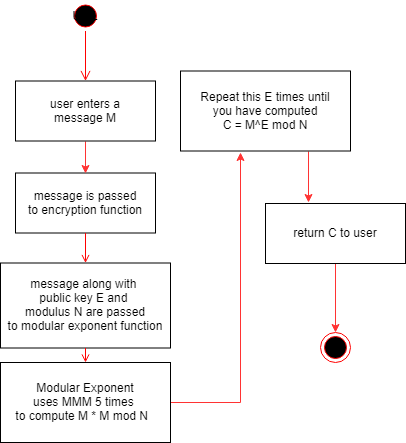
\includegraphics[scale=1]{UML1}

\clearpage

The second chart is a use case chart showing how Bob might send an encrypted message to Alice. First, Alice generates an RSA key-pair and gives Bob the public key N (the modulus) and E (the exponent). Next, Bob encrypts M under N and E and gives Alice the ciphertext C. Alice then uses her private key, D, to decrypt C and retrieves the message, M.

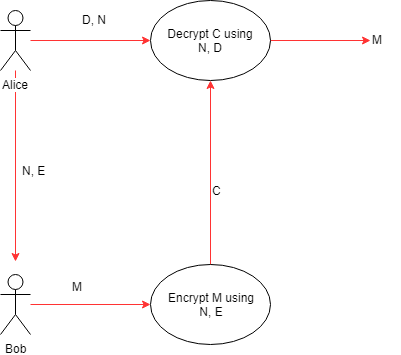
\includegraphics[scale=1]{UML2.png}


\end{document}
